	\section{Specifications}
	\subsection{Calculations}

	\subsubsection{Resolution and LSB}
	mapping 20Vpp Voltage space to a resolution of 16bit
	\begin{itemize}
		\item 0 ... 30000 ... 60000
		\item 1000 ... 31000 ... 61000
		\item 0 ... 32767 ... 65535
		\item ???
	\end{itemize}
	$\rightarrow$ LSB \^{=} ...mV


	\subsubsection{Trigger-Lines and Timers}
	utilisation of the output compare - timers
	\begin{itemize}
		\item TrigA \^{=} $TRIG\_2$  \^{=} PB3 $\leftarrow$ $TIM2_CH2$
		\item TrigB \^{=} $EN\_3$    \^{=} PC6 $\leftarrow$ $TIM8_CH1$
		\item TrigC \^{=} $EN\_4$    \^{=} PC7 $\leftarrow$ $TIM3_CH2$
	\end{itemize}

	\subsubsection{Triggers and Voltage - Outputs}
	association of Triggers and their analogue outputs
	\begin{itemize}
		\item TriggerB $\rightarrow$ SourceB $\rightarrow$ Vout1
		\item TriggerA $\rightarrow$ SourceA $\rightarrow$ Vout2
	\end{itemize}



	\subsection{FSM, FW-Struct}
		\begin{figure}[H]
			\center
			\includegraphics[width=0.75\textwidth]{src/_mainFSM_neato.pdf}
			\caption{Overarching finite-state-machine.}
			\label{fig:FSM}
		\end{figure}


		\begin{figure}[H]
			\center
			\includegraphics[width=0.75\textwidth]{src/_FW-Modules.pdf}
			\caption{Modular structure.}
			\label{fig:_FW-Modules}
		\end{figure}
	

		% \begin{figure}[ht]
			% \centering
			% 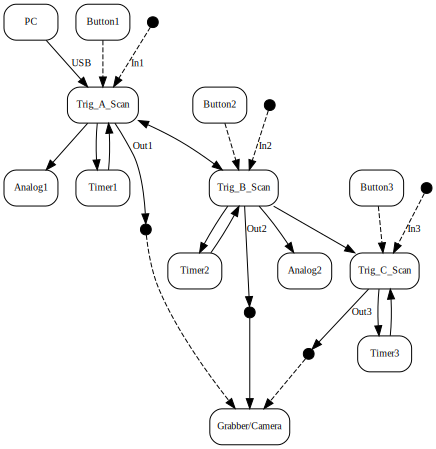
\includegraphics[height=105mm]{src/_Octane_Trigger_extended.pdf}
			% \caption{Trigger-structure.}
			% \label{_Octane_Trigger_extended}
		% \end{figure}

		\begin{figure}[ht]
			\centering
			\includegraphics[height=105mm]{src/_Octane_HW-Structure.pdf}
			\caption{Structure of the underlying hardware}
			\label{_Octane_HW-Structure.pdf}
		\end{figure}

% \spec{tag}{title}{module}{desc}
% \spec{}{}{}{}

	\spec{RI-}{Modules}{General}
	{ The Firmware has to be partitioned into these Modules:
		\begin{itemize}
		\item Main (Errorhandling)
		\item Triggers	(Timers)
		\item Sources	(SPI)
		\item Debug-Unit
		\item obs? System (WDG,CRC) 
		\item FSM (SCPI) 
		\item USB
		\item ResourceManager
		\item HAL (GPIO,WDG,CRC,DIO,UART,I2C,AIN)
		\item obs? Misc	(DIO,UART,I2C,AIN)
		\end{itemize}
	}

	\spec{RI-}{FSM-Module}{Main}
	{	the main-FSM has to implement the following functions
		\begin{itemize}
			\item 	uint8_t mainFSM() return 0 ... powerdown, -1 error, 1 ... reset, 2 ... restart
			\item 	bool parametrize(SCPI-ID, char * scpiString)
			\item 	bool processScpiID(SCPI-ID, char * scpiString)
		\end{itemize}
	}

	\spec{RI-}{FSM-States}{Main}
	{	the main-FSM has to implement the following states
		\begin{itemize}
		\item init
		\item running
		\item armed
		\item idling
		\item parametrizing 
		\item txUSB
		\item rxUsb
		\item errorState
		\end{itemize}
	}

	\spec{RI-}{ResMan}{General}
	{ All init()-Functions must probe the ResMan and only take and use a Resource when free. All deinit() - Functions must release Resources.}

	\spec{RI-}{Source-Modules}{Signals}
	{	16Bit-Voltage-Sources have to be accessible by following functions:
		\begin{itemize}
		\item 	\lstC !init() // not sure if necessary!
		\item 	\lstC !sendWord(bool source, uint16_t word)		// send 16Bit value over SPI to analog output!
		\item 	\lstC !loadArb(bool source, uint16_t size)!
		\item 	\lstC !scaleArb(bool source, uint16_t high, uint16_t low)! // rescale signal-vector vertically
		\item 	\lstC !loadRamp(bool source, uint16_t size, uint16_t high, uint16_t low)!
		\item 	\lstC !enab/disab analogue outputs A or B!
		\item 	\lstC !deinit() // not sure if necessary!
		\end{itemize}

		and following helper functions:
		\begin{itemize} \setlength\itemsep{1px}
			\item 	\lstC !float word2volt(uint16_t word) !
			\item 	\lstC !uint16_t	volt2word(float voltage) // -10V -> 0x00, 0 -> 30000, +10V -> 60000!
		\item 
		\end{itemize}

		and structures holding following data:
		\begin{itemize} \setlength\itemsep{1px}
		\item SPIx
		\item signalVector
		\item mode (triggered, detached, sinlgeshot)
		\item word min // upper vert. limit of ramp/arb
		\item word max // lower vert. limit of ramp/arb
		\item uint32	pulseTime
		\item 
		\end{itemize}
		
	}

	\spec{RI-}{scaling signals}{Signals}
	{	Vertically scaling of signal vectors will be applied irreversibly to signal-vectors in place.
		Amplitude, offset, high- and low-voltages are to be converted into min- and max-word and these again calculated onto existing vector values.
	}

	\spec{RI-}{writing signals}{Signals}
	{	Writing an arbitrary signal vector is only permitted in 'arbitrary'-mode. 
		Writing an arbitrary signal vector is complete if sufficient values were submitted and accepted.
		Writing an arbitrary signal vector can be aborted by setting the Sources mode to 'ramp'.
	}

	\spec{ RI- }{ResMan}{General}
	{ The FirmWare has to perform resource-management. This denotes to sanity-check managed resources being used by functionalities and deny functions if usage of resources would overlap.}

	\spec{ RI- }{ResourceList}{General}
	{ List of Resources to be managed:
		\begin{itemize} \setlength\itemsep{2px}
			\item Analogue Outputs, including SPIs, enable-Pins
			\item Analogue Inputs
			\item Digital Inputs/Outputs
			\item UART-Port
			\item I2C-Port
			\item Debug-Unit
			\item all processor-pins
		\end{itemize}
	}

	\spec{ RI- }{Debug-Unit}{Main}
	{ The Firmware has to implement a Debug-Unit, 8 digital outputs, that can be used to signalize certain events by setting/resetting/toggling them.
		Required functions are 
		\begin{itemize} \setlength\itemsep{1px}
		\item \lstC !initDbgUnit(void)  !
		\item \lstC !setDbgPinX(void)   !
		\item \lstC !clrDbgPinX(void)   !
		\item \lstC !tglDbgPinX(void)   !
		\item \lstC !deinitDbgUnit(void)!
		\end{itemize}
	}

	\spec{ RI- }{USB-Transceiver}{USB}
	{ The Firmware has to implement a USB-Transceiver for string-messages via VCP/CDC. Endpoints, to send and receive data have to established, as well as functions to access these endpoints.
		Required functions are 
		\begin{itemize} \setlength\itemsep{1px}
		\item \lstC !uint8_t CDC_Transmit_FS(uint8_t* Buf, uint16_t Len);!
		\item \lstC !// static int8_t CDC_Init_FS(void);!
		\item \lstC !// static int8_t CDC_DeInit_FS(void);!
		\item \lstC !// static int8_t CDC_Control_FS(uint8_t cmd, uint8_t* pbuf, uint16_t length);!
		\item \lstC !static int8_t CDC_Receive_FS(uint8_t* pbuf, uint32_t *Len);!
		\item \lstC !uint8_t newRxUSB(void);!
		\item \lstC !uint32_t lenRxUSB(void);!
		\item \lstC !void 	clrRxUSB(void);!
		\item \lstC !uint8_t *	getRxUSB(void);!
		\item \lstC !bool txUsb()!
		\item \lstC !initUsb()!
		\item \lstC !suspendUsb()!
		\item \lstC !resumeUsb()!
		\item \lstC !deinitUsb()!

		\end{itemize}
	}

	\spec{ RI- }{HAL-Module}{  }
	{ A hardware abstraction layer (HAL) has to be implemented, providing access to all necessary IO-Lines, serial-peripherals, the watchdog timer, cyclic-redundancy-check
	}

	\spec{ RI- }{HAL-Module}{  }
	{	must provide following interfacing functions:
		\begin{itemize} \setlength\itemsep{1px}
		\item initGPIOS()
		\item setPin()
		\item rstPin()
		\item getPin()
		\item deinitGPIOS()

		\item 
		\item initWDG(mode)
		\item setWDGtimeout()
		\item deinitWDG()

		\item initCRC()
		\item bool rxCRC(char * )
		\item txCRC(char * )
		\item deinitCRC()

		\item AIN, I2C, UART, DIO,
		\end{itemize}
		and following helper functions:
		\begin{itemize} \setlength\itemsep{1px}
		\item 
		\end{itemize}

		and structures holding following data:
		\begin{itemize} \setlength\itemsep{1px}
		\item 
		\end{itemize}

	}


	\spec{RI-}{scpi detection}{}
		{Implement USB-protocol in rSCPI.h, separately in short/longform, as well as an enum, representing the index of every command in the LUT.
		In the USB-ISR only mapping of the recieved string to a global variable and signaling to the FSM in main, that new data is to be processed happens, as well as sending out eventual Strings via USB.
		SCPI parsing in the FSM: looping over the SCPI-LUT and strncmp it to the input, until positive. Then either execute command immediately, or sscanf in the data. }

	\spec{}{scpi case-insensitive}{USB}
	{	\lstC !strncascmp()! ensures, that scpi-commands are detected case-insensitive
	}

	\spec{RI-}{thread-safe vriables}{main}{	Signalling between the FSM and the ISRs have to be thread-safe, and are therefore done via atomic operations, for example flags, semaphores or mutexes.
		Larger quantities of shared data, e.g. the signal vectors, are to be written, when the according ISR is deactivated, and may not be written on, while ISRs might read them. }

		\begin{figure}[ht]
			\centering
			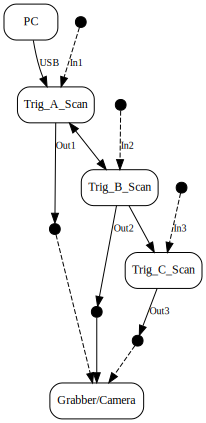
\includegraphics[height=105mm]{src/_Octane_Trigger_basic.pdf}
			\caption{Trigger-structure, basic concept.}
			\label{_Octane_Trigger_basic}
		\end{figure}
		\begin{figure}[ht]
			\centering
			\includegraphics[height=105mm]{src/_Octane_Trigger_extended_neato.pdf}
			\caption{Trigger-structure, extended concept.}
			\label{_Octane_Trigger_extended_kfdp}
		\end{figure}

	\spec{ RI- }{Naming Conventions}{ General }
	{	The following conventions shall be applied:
		\begin{itemize} \setlength\itemsep{1px}
		\item camelCase
		\item acting-Functions: 'verbNoun()'
		\item binary queries: 'is...()'
		\item 
		\end{itemize}
	}

	\spec{RI-}{naming convention}{General}
	{	naming scheme for digital IOs:
		\begin{itemize} \setlength\itemsep{1px}
			\item void	set<PinXY>();
			\item void	clr<PinXY>();
			\item bool	get<PinXY>();
		\end{itemize}
		e.g.:
		\begin{itemize} \setlength\itemsep{1px}
		\item void	setEN3();
		\item void	clrLED3();
		\item bool	getGPIO7();
		\end{itemize}
	}

	\spec{ RI- }{third party libs}{  }
	{	\begin{itemize} \setlength\itemsep{1px}
		\item CMSIS - ARM CoreM4 - Libraries
		\item stdbool.h
		\item usbdcdcif.h
		\item STM32F4 Pin- and Register-Defines
		\end{itemize}
	}


\begin{verbatim}
	
	K:\FH\MA\wim.txt durchforsten
	
	enums
		SourceA|B
		TrigA|B|C
	vars
	
	* Module:
		TestCases: mirror all the functionalities requested by User-requirements
		HAL Buttons, GPIOs, Relays, LEDs
		Miscellaneous - AnalogIN: Burst-mode wo ADCs die DAC-vektoren missbrauchen?
						- DIO
						- UART
						- I2C
		System	CRC, Wdg, Pwd/Rest/Rese/...

\end{verbatim}
	\spec{ RI- }{}{  }
	{	
	}

	\spec{ RI- }{opt pausing of Triggers}{  }
	{	Optional functionality: a falling Edge on a Trigger-In or pushing a dedicated Button (at red LED) during the running state, pauses or stops a whle Trigger-Sequence
	}

	\spec{ RI- }{rxUSB and parametrizing}{ USB-Stack }
	{	upon recieving a valid USB-packages, a parametrizazion-procedure has to be executed:
		validieren, applizieren, module updaten (Timers, Vektoren, Miscs ....)
		parametrize() - functions sits within the FSM Module and holds the long list of scpiID -> functions-calls
	}

	\spec{ RI- }{ISRs}{  }
	{	Necessary ISRs:
		\begin{itemize} \setlength\itemsep{1px}
		\item Buttons
		\item Timers for Triggers
		\item Trigger-Inputs
		\item UART, I2C, SPI
		\item USB
		\item Timer for Debounce
		\item Timer for Timeouts
		\end{itemize}
	}

	\spec{ RI- }{USB - safety}{  }
	{	USB-Inputs have to be sanity-checked regarding frequency, length and meaningful messages, as well as parameters within specified ranges

	}

	\spec{ RI- }{avoid reach-through}{ General }
	{	Timers, purposed for Triggers, are only to be accessed by their corresponding Trigger-unit.
		SPI-Ports are only to be accessed via their corresponding Source-Units.
	}

	\spec{ RI- }{ISR names}{ IRQs }
	{	Are defined in 'startup.....s'-assembler-file.	}

	\spec{ RI- }{Timer units}{ Timer }		% 2,8,3
	{	must provide following interfacing functions:
		\begin{itemize} \setlength\itemsep{1px}
			\item \lstC !bool initTimer(TIM_TypeDef * TIMx) // generic init to PWM-mode, no parameters!
			\item \lstC !bool setTimer(TIM_TypeDef * TIMx, uint32_t PSC, uint32_t ARR, uint32_t Pulse, uint32_t count)!
			\item \lstC !void startTimer(TIM_TypeDef * TIMx) enable IRQ!
			\item \lstC !void pauseTimer(TIM_TypeDef * TIMx) disableIRQ!
			\item \lstC !void stopTimer(TIM_TypeDef * TIMx) ?= reset(void) // pause(), reset counters, clearPin, zeroDAC()!
			\item \lstC !void deinitTimer(TIM_TypeDef * TIMx)	// generic deactivation of module!
			\item \lstC !void ISRs(void)!
		\end{itemize}
		and following helper functions:
		\begin{itemize} \setlength\itemsep{1px}
			\item timeStruct timerLUT(period)
			\item timeStruct timerHybrid(period) ... get PSC from LUT, calc ARR and pulse 
			\item $t_{samp}  = \frac{((PSC + 1)*(ARR+1))}{TCLK}$ -> $PSC = \frac{t_{samp} * TCLK }{(ARR+1)} - 1$
			% \item -> $t_{sampmin}  = \frac{((PSC + 1)( 0 + 1))}{TCLK} -> PSC + $
			% \item -> $t_{sampmax}  = \frac{((PSC + 1)( 2^{16} + 1))}{TCLK}$
			\item 	PSC-LUT: Zeitbereiche innerhalb derer ein PSC gilt, tmin $ = ((PSC + 1)*(0+1))/CLK$, tmax = $((PSC + 1)*(2^16+1))/CLK$ 
				\item 	jeder Eintrag in PSC-LUT ist eine union aus iTmin, iTmax, oPSC. timerHybrid() schleiferlt da drueber, bis passender \item 	PSC gefunden und rechnet daraus ARR und pulse
			\item timeStruct timerCALC(period) // timerFreq = Fclk/((PSC + 1)(ARR+1))
			\item $uint32\_t$ getTimerPSC(period) // LUT calculating PSC from given Timer-period: 0 for 4us ... 
		\end{itemize}

		and structures holding following data:
		\begin{itemize} \setlength\itemsep{1px}
		\item 	timeStruct: 	ARR, PSC, CCRx, ?length?
		\end{itemize}
	}

	\spec{ RI- }{Trigger units}{  }
	{	must provide following interfacing functions 
		\begin{itemize} \setlength\itemsep{1px}
		\item bool init(TRIG-ID, length, period, mode/input, , ...)
		\item arm(TRIG-ID)
		\item run(TRIG-ID) = start(TRIG-ID)
		\item pause(TRIG-ID)
		\item stop(TRIG-ID)
		\item reset(TRIG-ID)
		\item deinit(TRIG-ID)
		\end{itemize}

		and following helper functions:
		\begin{itemize} \setlength\itemsep{1px}
		\item nix, weil Timing in den Timer-Units berechnet wird
		\end{itemize}

		and structures holding following data:
		\begin{itemize} \setlength\itemsep{1px}
		\item TRIG-ID, TIM-ID
		\item state
		\item length, signal-period = time = 1/rate = 1/freq
		\item input/event-source
		\end{itemize}
	}

	\spec{ RI- }{ ResourceManager }{ Main }
	{	must provide following interfacing functions:
		\begin{itemize} \setlength\itemsep{1px}
		\item bool isTaken( <ResENUM> )
		\item bool take( <ResENUM> )
		\item void release( <ResENUM> )
		\end{itemize}
		and following helper functions:
		\begin{itemize} \setlength\itemsep{1px}
		\item 
		\end{itemize}

		and structures holding following data:
		\begin{itemize} \setlength\itemsep{1px}
		\item 	\lstC !ResENUM	{ RES_ 	RES_TRIGA 	RES_TRIGB 	RES_TRIGC 	RES_SOURCEA 	RES_SOURCEB 	RES_GPIO_E 	RES_UART 	
					  RES_I2C 	RES_SPI 	RES_ADC 	RES_Relay 	RES_TIMx 	RES_TIMx 	RES_TIMx 	RES_TIMx	RES_		}!
		\item 			Ausschlusstabelle zw Pins
		\end{itemize}
	}
			
	\spec{ RI- }{SPI units}{  }
	{	must provide following interfacing functions:
		\begin{itemize} \setlength\itemsep{1px}
		\item bool initSPI(SPIx) (in 16Bit Mode)
		\item txSpi(SPIx, word )
		\item word rxSpi(SPIx)
		\item deinitSPI(SPIx)
		\end{itemize}
		and following helper functions:
		\begin{itemize} \setlength\itemsep{1px}
		\item 
		\end{itemize}

		and structures holding following data:
		\begin{itemize} \setlength\itemsep{1px}
		\item 
		\end{itemize}

	}

	\spec{ RI- }{SCPI Module}{  }
	{	must provide following interfacing functions:
		\begin{itemize} \setlength\itemsep{1px}
		\item word getIDfromSCPIstring(char * scpiString, uint16 strLen)
		\end{itemize}

		and structures holding following data:
		\begin{itemize} \setlength\itemsep{1px}
		\item Stringlists containing recendt-shorts and -longs and norm-commands
		\item enum with exact same order as stringlists
		\item OR: \lstC !struct {longform, shortform, ID}! and for every ID a  \lstC !#define 0 TRIGA_STATE_OFF!
		\end{itemize}
	}

	% \spec{ RI- }{ units}{  }
	% {	must provide following interfacing functions:
		% \begin{itemize} \setlength\itemsep{1px}
		% \item init()
		% \item deinit()
		% \end{itemize}
		% and following helper functions:
		% \begin{itemize} \setlength\itemsep{1px}
		% \item 
		% \end{itemize}

		% and structures holding following data:
		% \begin{itemize} \setlength\itemsep{1px}
		% \item 
		% \end{itemize}

	% }

	\spec{ RI- }{Main module}{ Main }
	{	The firmware has to implement a main-Module, initializing all permanent modules (System-Clock, USB), activate the main-FSM and execute error-handling. It must provide following functions:
		\begin{itemize} \setlength\itemsep{1px}
		\item main(), including a super-loop and a call to the mainFSM
		\item ErrorHandler()
		\end{itemize}
		
		and structures holding following data:
		\begin{itemize} \setlength\itemsep{1px}
		\item scpi-identification string
		\item Processor Clock
		\item 
		\item 
		\end{itemize}

	}




	\spec{ RI- }{SysTick}{ main }
	{	A SysTick has to be established with a period of 10ms $\mu$s .
	}

	\spec{ RI- }{Clock}{ main }
	{	The Processor has to run at a frequency of 96MHz.
	}

	\spec{ RI- }{ms-Delay}{ main }
	{	The FW has to implement a loosely timed Delay function 
		\lstC !void delay_ms(int ms){     uint32 start=systickcount;    while (systickcount-start<ms); }!
	}

	\spec{ RI- }{Finite State Machine}{ main }
	{ The FW has to implement an event-driven FSM, that handles the necessary states, transitions and events according to figure \ref{fig:FSM} }

	\spec{ RI- }{LUT Signals}{ todo }
	{ The FW shall implement look-up-tables, 2 vectors, one for each Generator-channel, each at least of 2\textsuperscript{16} words(16bit) length, to contain user-defined waveforms for the Analog Outputs }

	\spec{ RI- }{Relais abstractions \label{relais}}{ todo }
	{ The FW shall implement functions to access relais, providing 'turn on', 'turn off' and 'retrieve status' }

	\spec{ RI- }{Abstraction of SignalGenerator-HW \label{absSigal}}{ todo }
	{ The FW shall implement functions to access the analog outputs, relying on the SPI-abstraction provided by REQ\ref{absFast} Enabling/disabling specified channels, setting specified voltage values.		}

	\spec{ RI- }{Abstraction of onboard-analogs \label{absADC}}{ todo }
	{ desc }

	\spec{ RI- }{Abstractions of highspeed digital IOs \label{absFast}}{ todo }
	{ The FW shall implement functions to manipulate and read the states of the Trigger IOs and SPI-channels and also to define them as outputs (initially), or inputs.}

	\spec{ RI- }{Abstractions of lowspeed digital IOs \label{absSlow}}{ todo }
	{ The FW shall implement functions to manipulate and read the states of the enable-lines of analog-outputs, and relay-lines and also to define them as outputs }

	\spec{ RI- }{Abstractions of misc. digital IOs }{ todo }
	{ The FW shall implement functions to manipulate and read the states of Buttons, Status-LEDs, Port3(8IOs), Port5(16IOs)  and also to define them as outputs (initially), or inputs. }

	\spec{ RI- }{ISR}{ General }
	{ The FW has to implement ISR-callbacks, to notice trigger-events on Button/Ext TriggerA...D, ISRs for TimersA,B and C, USBrx, ?USBtx? }

	\spec{ RI- }{Encoder/Stepper}{ todo }
	{ optional: The Firmware has to access available hardware to read encoder signals and send stepper commands. }

	\begin{table}[ht!]
	\centering
	\begin{tabular}{|l|c|l|l|l|l|}
	\hline
	\redrow Module	& Prio & Type	& Size 	& Purpose		& initial value \\ \hline
	% \hhline{======}                         	
	FSM			& H	& struct	& 			& 					& 		\\ \hline
			% 	& M	& enum		& -			& statePrev			& INIT	\\ \hline
				& H	& enum		& -			& state				& INIT	\\ \hline
				& M	& enum		& -			& stateNext			& INIT	\\ \hline
				& H	& flag		& -			& inUSBnew			& low	\\ \hline
				& H	& flag		& -			& outUSBnew			& low	\\ \hline
	USB-Stack	& H	& struct	& 			& 					& 		\\ \hline
				& H	& string	& 			& inUSB				& empty	\\ \hline
				& H	& string	& 			& outUSB			& empty	\\ \hline
				& H	& 			& 			& max. String lenght		& 		\\ \hline
	SCPI		& H	& 			& 			& 					& 		\\ \hline
				& H	& str-list	& 			& SCPI commands	lon & 		\\ \hline
			%	& H	& str-list	& 			& SCPI commands	sho & 		\\ \hline
				& H	& str-list	& 			& SCPI responses	& 		\\ \hline
				& H	& str-list	& 			& error codes		& 		\\ \hline
				& H	& enum		& 			& command coding	& 		\\ \hline
	Trigger A	& H	& struct	& 			& 					& 		\\ \hline
	Trigger B	& H	& struct	& 			& 					& 		\\ \hline
	Trigger C	& H	& struct	& 			& 					& 		\\ \hline
	Generator 1	& H	& struct	& 			& 					& 		\\ \hline
				& H	& 16 bit	& $>2^{16}$	& Signal-Vector		& 0s	\\ \hline
	Generator 2	& H	& struct	& 			&					& 		\\ \hline
				& H	& 16 bit	& $>2^{16}$	& Signal-Vector		& zeroes\\ \hline
	Relais 1..8	& H	& structs	& 			& 					& 		\\ \hline
	Watchdog	& H	& struct	& 			& 					& 		\\ \hline
	CRC			& H	& struct	& 			& 					& 		\\ \hline
	IO-Lines	& H	& structs	& 			& 					& 		\\ \hline
	% Peripherals	& H	& structs	& 			& 					& 		\\ \hline
			\end{tabular}
		\caption{Required data inside the FW.}
	\label{tab:Vars}
	\end{table}
	
	\spec{RI-}{how to Trigger}{Triggers}
	{	\begin{itemize}
		\item A Trigger Event is either a SCPI-Command "TRIGx:STAT:RUN", an external logic Signal on signal-line TRIGx, or by pressing the button BUTTx, or, in linked mode, issued by the superior Trigger. 
		\item A Trigger Event causes the according Timer-Interrupt to be enabled. The affected Trigger-unit then, runs for a number of steps specified by "TRIGx:COU count", with a speed defined by "TRIG0:TIME time" or "TRIGx:FREQ freq", and after that disables its own Interrupt. 
		\item Activation of at least one Trigger causes the USB-Interrupt to be deactivated, to ensure no interference with the critical timing of Triggering and Signal Generation. Unless Trigger a or B have a duration of at least 2 seconds, or at least one Trigger has a Step-Count of '0',in which case USB-Interrupt needs to be active, otherwise, the whole OCTane would be frozen for too long. 
		\item Every step, the Trigger pulses its own Trigger-Output line, reads the recent value from its Generators LUT and sends that value to the Gen via SPI, increases the step count and potentially triggers its inferior Trigger. 
		\item In linked mode, the superior unit enables the IRQ of the inferior. In independent mode, a button, an ext Trigger, or the SCPI-Command triggers an IRQ. 
		\end{itemize}
	}

		\begin{table}[H]
			\centering
			\begin{tabular}{|l|l|l|l|l|l|}
			\hline
			\redrow Function		& Prio 	& Port	& HW-Identifier 			& Type	& initial value \\ \hline
					Trigger 1		& high 	& A		& $TRIG\_1$	& digital IO, HighSpeed		& low		\\ \hline
					Trigger 2		& high 	& B		& $TRIG\_2$	& digital IO, HighSpeed		& low		\\ \hline
					Trigger 3		& high 	& B		& $TRIG\_3$	& digital IO, HighSpeed		& low		\\ \hline
					Trigger 4		& high 	& B		& $TRIG\_4$	& digital IO, HighSpeed		& low		\\ \hline
					SPI 1			& high 	& A		& $SCLK\_1, NSS\_1, MISO\_1, MOSI\_1$	& Serial Peripheral IF, HighSpeed		& 0x0000		\\ \hline
					SPI 2			& high 	& B		& $SCLK\_2, NSS\_2, MISO\_2, MOSI\_2$	& Serial Peripheral IF, HighSpeed		& 0x0000		\\ \hline
					Relais, SLD		& high 	& D		& $GPIO\_8$	& digital out, LowSpeed		& low		\\ \hline
					Relais, AIM		& high 	& D		& $GPIO\_7$	& digital out, LowSpeed		& low		\\ \hline
					Relais, CAM		& high 	& D		& $GPIO\_6$	& digital out, LowSpeed		& low		\\ \hline
					Relais, Galvo	& high 	& D		& $GPIO\_5$	& digital out, LowSpeed		& low		\\ \hline
					State LED, 1	& low 	& D		& $STATE\_1$	& digital out, LowSpeed	& low		\\ \hline
					State LED, 2	& low 	& D		& $STATE\_2$	& digital out, LowSpeed	& low		\\ \hline
					State LED, 3	& low 	& D		& $STATE\_3$	& digital out, LowSpeed	& low		\\ \hline
					State LED, 4	& low 	& D		& $STATE\_4$	& digital out, LowSpeed	& low		\\ \hline
					PushButton, 1	& mid 	& D		& $BUTT\_1$	& digital in, LowSpeed			& n.a.		\\ \hline
					PushButton, 2	& mid 	& D		& $BUTT\_2$	& digital in, LowSpeed			& n.a.		\\ \hline
					PushButton, 3	& mid 	& D		& $BUTT\_3$	& digital in, LowSpeed			& n.a.		\\ \hline
					PushButton, 4	& mid 	& D		& $BUTT\_4$	& digital in, LowSpeed			& n.a.		\\ \hline
					enable Analog1	& high 	& C		& $EN\_1$	& digital out, LowSpeed		& low		\\ \hline
					enable Analog2	& high 	& C		& $EN\_2$	& digital out, LowSpeed		& low		\\ \hline
					Analog in 1		& low 	& C		& $ADC\_1$	& analog In		& n.a.		\\ \hline
					Analog in 2		& low 	& C		& $ADC\_2$	& analog In		& n.a.		\\ \hline
					Analog in 3		& low 	& C		& $ADC\_3$	& analog In		& n.a.		\\ \hline
					Analog in 4		& low 	& C		& $ADC\_4$	& analog In		& n.a.		\\ \hline
					USB				& high 	& -		& $USB\_FS\_DM$	& USB Data-		& n.a.		\\ \hline
					USB				& high 	& -		& $USB\_FS\_DP$	& USB Data+		& n.a.		\\ \hline
					USB				& high 	& -		& $USB\_FS\_ID$	& USB ident.	& n.a.		\\ \hline
					\end{tabular}
					\caption{Mapping of IO-lines.}
					\label{tab:Mapping}
		\end{table}

